\documentclass[conference]{IEEEtran}
\IEEEoverridecommandlockouts
% The preceding line is only needed to identify funding in the first footnote. If that is unneeded, please comment it out.
\usepackage{cite}
\usepackage{amsmath,amssymb,amsfonts}
\usepackage{graphicx}
\usepackage{amsmath}
\usepackage[ruled,linesnumbered,vlined]{algorithm2e}
\usepackage{textcomp}
\usepackage{xcolor}
\usepackage{ifpdf}
\usepackage{epsfig,graphicx}
\usepackage{float}
\usepackage{algorithm,algorithmic}
\usepackage{microtype}
\usepackage{mathtools}
\usepackage{amssymb,amsmath,epsfig, graphics,floatflt}
\usepackage{comment}
\pagestyle{empty}
\usepackage{amsmath}
\usepackage{subfigure}
\usepackage{array}
\usepackage{fixltx2e}
\usepackage{subcaption}
\usepackage[labelformat=parens,labelsep=quad,skip=3pt]{caption}
\usepackage{url}
\DeclareCaptionLabelFormat{plain}{#1 #2}
\captionsetup[figure]{labelformat=plain}
\def\BibTeX{{\rm B\kern-.05em{\sc i\kern-.025em b}\kern-.08em
    T\kern-.1667em\lower.7ex\hbox{E}\kern-.125emX}}
\begin{document}

\title{Edge-Intelligence based Federated Learning in the Internet of Medical Things}
\author{	\IEEEauthorblockN{Suresh Chavhan \IEEEauthorrefmark{1}, Beerelly Srinitha \IEEEauthorrefmark{1}, Sikander Kathat \IEEEauthorrefmark{1}, Ashit Kumar Dutta \IEEEauthorrefmark{2}, Joel J. P. C. Rodrigues\IEEEauthorrefmark{3}\\	}
\vspace{0.1in}
\IEEEauthorblockA{  \IEEEauthorrefmark{1}Department of Computer Science and Engineering,\\ Indian Institute of Information and Technology Raichur, Karnataka, India.\\
\IEEEauthorrefmark{2} Department of Computer Science and Information Systems, College of Applied Sciences,\\ AlMaarefa University, Ad Diriyah, Riyadh, 13713, Kingdom of Saudi Arabia.\\ 
\IEEEauthorrefmark{3} Amazonas State University, Manaus - AM, Brazil.\\ }
suresh@iiitr.ac.in, srinithabeerelly1905@gmail.com,  sikanderkat@gmail.com, adotta@um.edu.sa, and joeljr@ieee.org }

\maketitle

\begin{abstract}
In the evolving healthcare landscape, the Internet of Medical Things (IoMT) enables real-time data collection through connected devices. Concerns about data privacy in electronic health records are driving changes in health assessment. Blended learning is emerging as a solution, allowing simulation training without sharing critical information centrally. The proposed techniques emphasize privacy and efficiency and use federated averaging to analyze edge computation. Smart healthcare addresses the benefits and challenges of integrating AI and edge tech. In this revolutionary approach, federated learning uses server-side federated averaging, combining local client model parameters while reducing edge computation latency and energy consumption The integration of AI and edge technologies not only increases efficiency but also provides forward-looking approaches for personalized and responsive healthcare. Experimental validation with the Covid-pneumonia dataset highlights the effectiveness of the integrated learning approach, confirming the important contribution to privacy protection and efficient machine learning applications in computing in healthcare of the policies established in countries.

\textit{Keywords: Federated Learning, Decentralized Machine Learning, Computational Efficiency, Internet-of-Medical-Things, Edge Computing, Smart Healthcare Systems, Support Vector Machines.}


\end{abstract}

\section{Introduction}

Healthcare stands at the forefront of human welfare, and as the global population is expanding rapidly, the demand for healthcare services has reached unprecedented levels. Simultaneously, technological advancements, particularly the evolution of the Internet of Things (IoT) and advancements in wireless communications have ushered in a new era of healthcare known as smart healthcare\cite{1} or connected healthcare systems. Unlike conventional healthcare systems, smart healthcare leverages technologies such as IoT, wearable devices, and advanced communication protocols to create dynamic connections between patients, caregivers, and healthcare institutions. This interconnected ecosystem enables the seamless transfer of information, transforming the delivery of healthcare services. Smart healthcare services go beyond conventional medical approaches by intelligently handling and responding to medical requests remotely. This not only significantly reduces hospitalization rates but also empowers both individuals and healthcare professionals to predict, detect, diagnose, and intelligently treat diseases. Moreover, in the context of global health challenges, smart healthcare plays a pivotal role in preventing and controlling the outbreak of contagious and infectious diseases like the COVID-19 pandemic.

To support the expansion of healthcare facilities and cater to the increasing user demands, smart healthcare systems integrate a myriad of smart devices and IoT technologies. This integration, however, results in the generation of a massive volume of heterogeneous medical records. Effectively processing and evaluating this data in real-time is imperative, especially in emergency cases where low response times are critical. The latency at centralized data centres poses risks that can lead to irreparable consequences, emphasizing the need for efficient communication among various entities in the smart healthcare community. As machine learning algorithms increasingly rely on data, the scalability and security challenges associated with centralized data repositories become apparent. Setting up and maintaining such infrastructure requires significant investment, and the risk of security breaches leading to data leaks poses serious concerns. Thus Federated Learning (FL) emerges as a solution to address these challenges by integrating and adopting edge computing technology and artificial intelligence (AI)\cite{2} in smart healthcare systems. Edge computing, with its capability to process data closer to its source, and AI, with its intelligent decision-making capabilities, offer a synergistic solution to enhance communication efficiency, reduce response times in smart healthcare systems, and enable collaborative model training across multiple client devices without the need to share local data. 

FL\cite{3} operates by training a shared model on a server using proxy data, after which participating devices perform local training and contribute to model improvement. Federated averaging is employed to aggregate model parameters from clients and calculate updated models. The iterative process continues until convergence is achieved, allowing for runtime scaling without the complexity of centralized systems. The application of FL\cite{4} is particularly relevant in these scenarios where data is sensitive, and restrictions on data sharing exist, making it suitable for industries such as healthcare, finance, and the Internet of Things. This work focuses on SVM-based models, chosen for their theoretical robustness, reduced risk\cite{5} of overfitting compared to neural networks, and minimal memory requirements on the client side.

In this paper, FL for a binary classification problem is implemented using Support Vector Machines (SVM) on the Covid-Pneumonia dataset, aiming to assess its performance. Although most FL research to date has used neural network designs, the selection of SVM has several advantages: it has a solid theoretical base, requires less memory, and requires less communication when exchanging model parameters. This study aims to assess the model's effectiveness and contrast its results with those of a centralized model.
In the context of IoMT\cite{6}, the advantages of FL can further be amplified when combined with the concept of sparsity. Sparse Federated Learning (SFL) is an emerging field that leverages the inherent sparsity in medical data. Medical data often contain redundant or irrelevant information, and sparse learning techniques aim to exploit this property for more efficient model training. The paper also discussed SFL which has a future scope to be worked on and enhance the capabilities of FL. This research aims to contribute to developing more secure and efficient healthcare systems that harness the power of IoMT while safeguarding patient privacy.

The rest of the paper is organized as follows. Section II comprehensively presents the related works. Section III presents the background. Section IV discusses the proposed solution. Section V shows the system architecture. Section VI discusses the mathematical model. The simulation scenario, dataset, results, and analysis are discussed in Section VII. Finally, conclusions and future works are drawn in Section VIII.



\section{Related Work}
Federated Learning (FL) and the Internet of Medical Things (IoMT)\cite{4}  represent two dynamically evolving fields at the intersection of healthcare, machine learning, and connected devices. This section provides an overview of the existing body of research that forms the foundation for the exploration into the integration of FL within IoMT ecosystems. Understanding the landscape of related works is crucial for contextualizing the contributions of this research, which seeks to address privacy concerns and scalability challenges in healthcare analytics.

% \subsection{Federated Learning in Healthcare}

Research in FL has made substantial contributions to healthcare applications, particularly in addressing privacy concerns associated with patient data. Studies have delved into the development of FL models tailored for healthcare scenarios. For instance, focused on disease prediction have leveraged decentralized learning to accommodate the sensitive nature of medical records.\cite{5} Additionally, personalized treatment recommendations and medical image analysis have been explored within the FL framework. These applications aim not only to enhance patient privacy but also to provide intelligent and personalized healthcare solutions.

% \subsection{Communication-Efficient FL}

Addressing communication challenges has been a focal point in FL research, especially concerning the interaction between clients and central servers. Studies have investigated techniques to reduce communication\cite{6} overhead and enhance efficiency. Quantization, model compression, and adaptive aggregation methods have been explored to optimize the communication process in FL. These innovations aim to minimize the impact of large-scale model updates on network bandwidth and improve the overall scalability of FL systems.

% \subsection{Privacy-Preserving Machine Learning}

A significant body of work has concentrated on fortifying privacy\cite{7} in machine learning, with FL emerging as a key player in this domain. Techniques such as secure aggregation and differential privacy have been explored extensively to ensure the protection of sensitive information. The implementation of secure aggregation protocols has enabled collaborative model training without compromising individual data privacy. Differential privacy mechanisms have been investigated to add an additional layer of privacy guarantees, making FL a robust solution for privacy-preserving machine learning across decentralized devices.

% \subsection{Security and Robustness in FL}
The development and refinement of FL frameworks have been crucial for advancing the field. TensorFlow Federated (TFF) and PySyft are notable examples of frameworks that facilitate the implementation of FL algorithms. TFF, in particular, provides a standardized platform for federated computations, allowing researchers to easily experiment with and deploy FL models. These frameworks have not only accelerated research but have also encouraged collaboration among researchers by providing shared platforms for experimentation and model development. Ensuring the security\cite{8} and robustness of FL models has been a paramount concern in research. Investigations have focused on mitigating adversarial attacks, a critical aspect given the decentralized nature of FL. Secure aggregation protocols have been designed to protect against potential attacks during the model aggregation phase. Additionally, techniques to handle Byzantine failures, where participating nodes act maliciously, have been explored to enhance the resilience of FL systems.

% \subsection{FL in Edge Computing}

The integration of FL with edge computing\cite{9} has garnered significant attention. This integration aims to enable model training and inference at the edge, addressing challenges related to latency and bandwidth constraints. By bringing computation closer to data sources, FL in edge computing seeks to enhance the efficiency of model updates and reduce the reliance on central servers. This is particularly crucial in scenarios where real-time decision-making is essential, such as in healthcare and IoT applications. Cross-silo FL, involving collaboration across multiple organizations or data silos, has been a research focus. This extends the applicability of FL to scenarios where data is distributed across diverse entities\cite{7}. Additionally, FL on mobile and IoT devices, where data is inherently decentralized, has emerged as a growing area of interest. Understanding the challenges and opportunities posed by diverse data distributions is vital for the successful implementation of FL across different silos and devices.

% \subsection{FL Applications in Various Domains}

Research in FL has expanded its applications to various domains beyond healthcare. Studies have explored the applicability of FL in finance, telecommunications, and industrial IoT. The emphasis has been on tailoring FL to meet the specific requirements and challenges of each domain. For instance, in finance, FL may be leveraged for collaborative predictive modelling without compromising sensitive financial data. These domain-specific applications underscore the versatility and potential impact of FL in addressing diverse data privacy\cite{8} and collaboration challenges. In conclusion, the related works in FL presented a comprehensive overview of advancements in privacy, communication efficiency, security, and applications across different domains. Ongoing research continues to refine and extend the capabilities of FL, making it a versatile and promising paradigm for decentralized machine learning. Researchers are encouraged to stay abreast of the latest developments in leading conferences and preprint repositories for the most recent insights into FL research.

\section{Background}

The confluence of Edge Computing, Artificial Intelligence (AI), the Internet of Medical Things (IoMT), and Federated Learning (FL) heralds a transformative era in healthcare, offering unprecedented opportunities for enhanced patient care, diagnostics, and analytics. This section provides a comprehensive background on each of these pillars and elucidates their integration to address the intricate challenges and opportunities in the healthcare landscape.

\subsection{Edge Computing}

Edge Computing is a decentralized computing paradigm that brings computation and data storage closer to the source of data generation. In healthcare, this means processing and analyzing data at the edge of the network\cite{2,10}, near medical devices and sensors, rather than relying solely on centralized cloud servers. In healthcare, the significance of Edge Computing lies in its ability to reduce latency, enhance real-time processing, and alleviate bandwidth constraints. By enabling data processing closer to where it is generated, Edge Computing supports time-sensitive applications critical for medical decision-making.

\subsection{Artificial Intelligence (AI)}

Artificial Intelligence refers to the simulation of human intelligence in machines, enabling them to perform tasks that typically require human cognition. In healthcare, AI encompasses machine learning, natural language processing, and computer vision, among other techniques \cite{9, 11, 12}. AI revolutionizes healthcare by automating diagnostics, predicting patient outcomes, and personalizing treatment plans. It aids in the analysis of vast datasets, facilitating more accurate and timely decision-making by healthcare professionals.

\subsection{Internet of Medical Things (IoMT)}

The Internet of Medical Things involves connecting medical devices and systems through the Internet to collect, share, and analyze health data. IoMT\cite{1} encompasses a wide array of devices, including wearables, sensors, and medical equipment. IoMT enhances patient monitoring, enables remote patient care, and facilitates the continuous collection of health data. It promotes proactive healthcare by providing real-time insights into patient conditions, leading to timely interventions and personalized treatment plans.

\subsection{Federated Learning (FL)}

Federated Learning is a machine learning approach where a model is trained collaboratively across decentralized edge\cite{3}  devices without centralizing raw data. Model updates occur locally, and only aggregated insights are transmitted to a central server.

\section{Proposed Solution}
The integration of Edge Computing, AI, IoMT, and FL is driven by the collective goal of enhancing healthcare analytics, patient outcomes, and operational efficiency. Edge Computing optimizes real-time processing, AI provides intelligent insights, IoMT connects diverse medical devices, and FL ensures privacy-preserving collaborative learning. The synergy between these technologies holds promise for personalized, efficient, and secure healthcare delivery. However, challenges such as interoperability, security, and ethical considerations necessitate a comprehensive understanding of their integration. FL addresses privacy concerns by allowing model training on local data without sharing sensitive information. In healthcare, where data privacy is paramount, FL offers a secure framework for collaborative model training across a network of distributed medical devices. In conclusion, the seamless integration of Edge Computing, AI, IoMT, and FL in healthcare represents a paradigm shift toward patient-centric, data-driven, and privacy-preserving healthcare systems. This research endeavours to explore the intricacies of this integration, addressing challenges and uncovering novel insights to propel healthcare into a new era of innovation and effectiveness using federated learning. It can be further improved in terms of communication cost by using sparsed federated learning where a mask is used to separate the important features and the unwanted features and only the important features are sent for global aggregation.

\section{System Architecture}
The construction of a global model using globally accessible proxy data is the first step in the Federated Learning architecture. On the server side, this model represents the current situation. To begin, each data holder requests the server's current model, which they then train using their local data. The server collects local model parameters regularly and uses them to improve the global model, updating all local sites. 

The server updates the global model by gathering model parameters from several sources and federatedly averaging them. This process keeps going until the model is saturated. Testing takes place both globally on a generic dataset and locally on the test set of each client. Variations in the properties of the data among tests may result in differences in the local and global test accuracies. The system architecture of the proposed model is shown in Fig. \ref{dis}

\begin{figure}[htp]
    \centering
    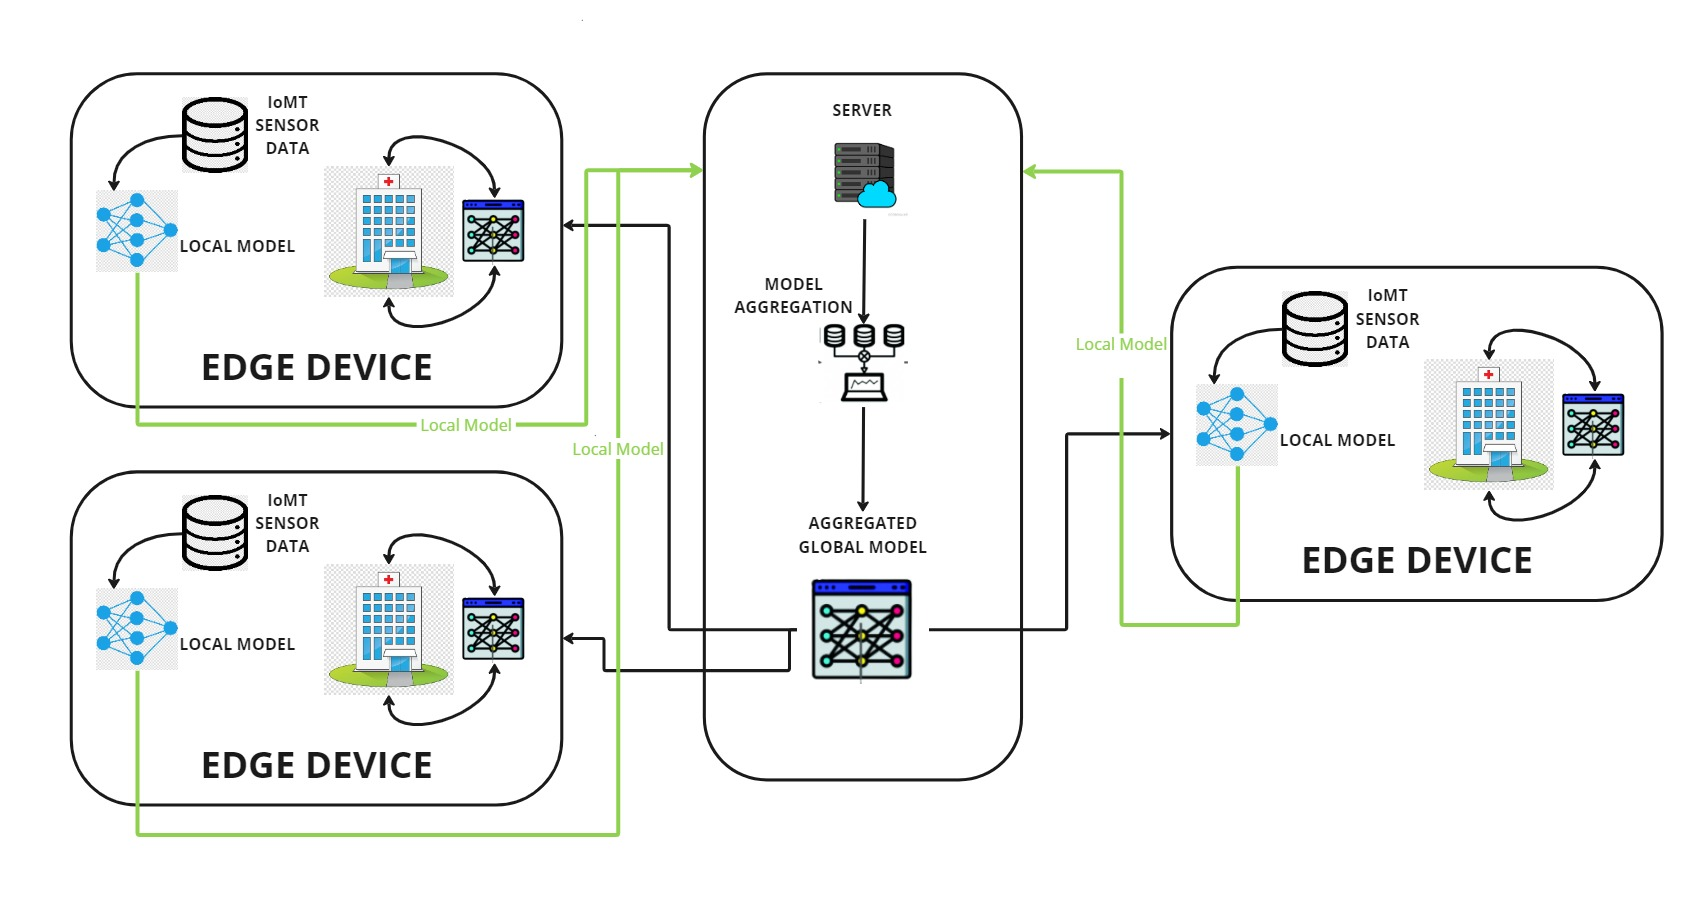
\includegraphics[scale = 0.14]{FL_ARCHITECTURE (3).jpg}
    \caption{Federated learning based System Architecture}
    \label{dis}
\end{figure}

In the realm of the Internet of Medical Things (IoMT), the benefits of Federated Learning (FL) can be significantly heightened by incorporating the concept of sparsity. Sparse Federated Learning (SFL) represents an emerging field that capitalizes on the inherent sparsity present in medical data. Medical datasets frequently encompass redundant or irrelevant information and sparse learning techniques are designed to capitalize on this property to facilitate more efficient model training.

Within the context of the research, discussing SFL as a prospective avenue for future work implies an acknowledgement of its current status as a developing field with considerable potential. The key idea is that sparse learning techniques when integrated into the federated learning framework, can enhance the overall efficiency and performance of the model.

In more detail, sparsity in medical data refers to the notion that not all elements or features within a dataset contribute equally to the learning process. Some information may be redundant or irrelevant to the task at hand. Sparse learning techniques, such as L1 regularization or feature selection, can be employed to identify and leverage this inherent sparsity. By focusing on the most informative features, these techniques aim to streamline the model and improve its generalization capabilities.

%The discussion of SFL as a future research direction implies an opportunity to dig deeper into how sparse learning techniques can be tailored specifically for the intricacies of medical data in federated settings. This might involve exploring novel algorithms or adapting existing sparse learning methods to the distributed and collaborative nature of federated learning in the medical domain. The architecture for the same can be modified as shown in Fig.\ref{ds}

%\begin{figure}[htp]
 %   \centering
  %  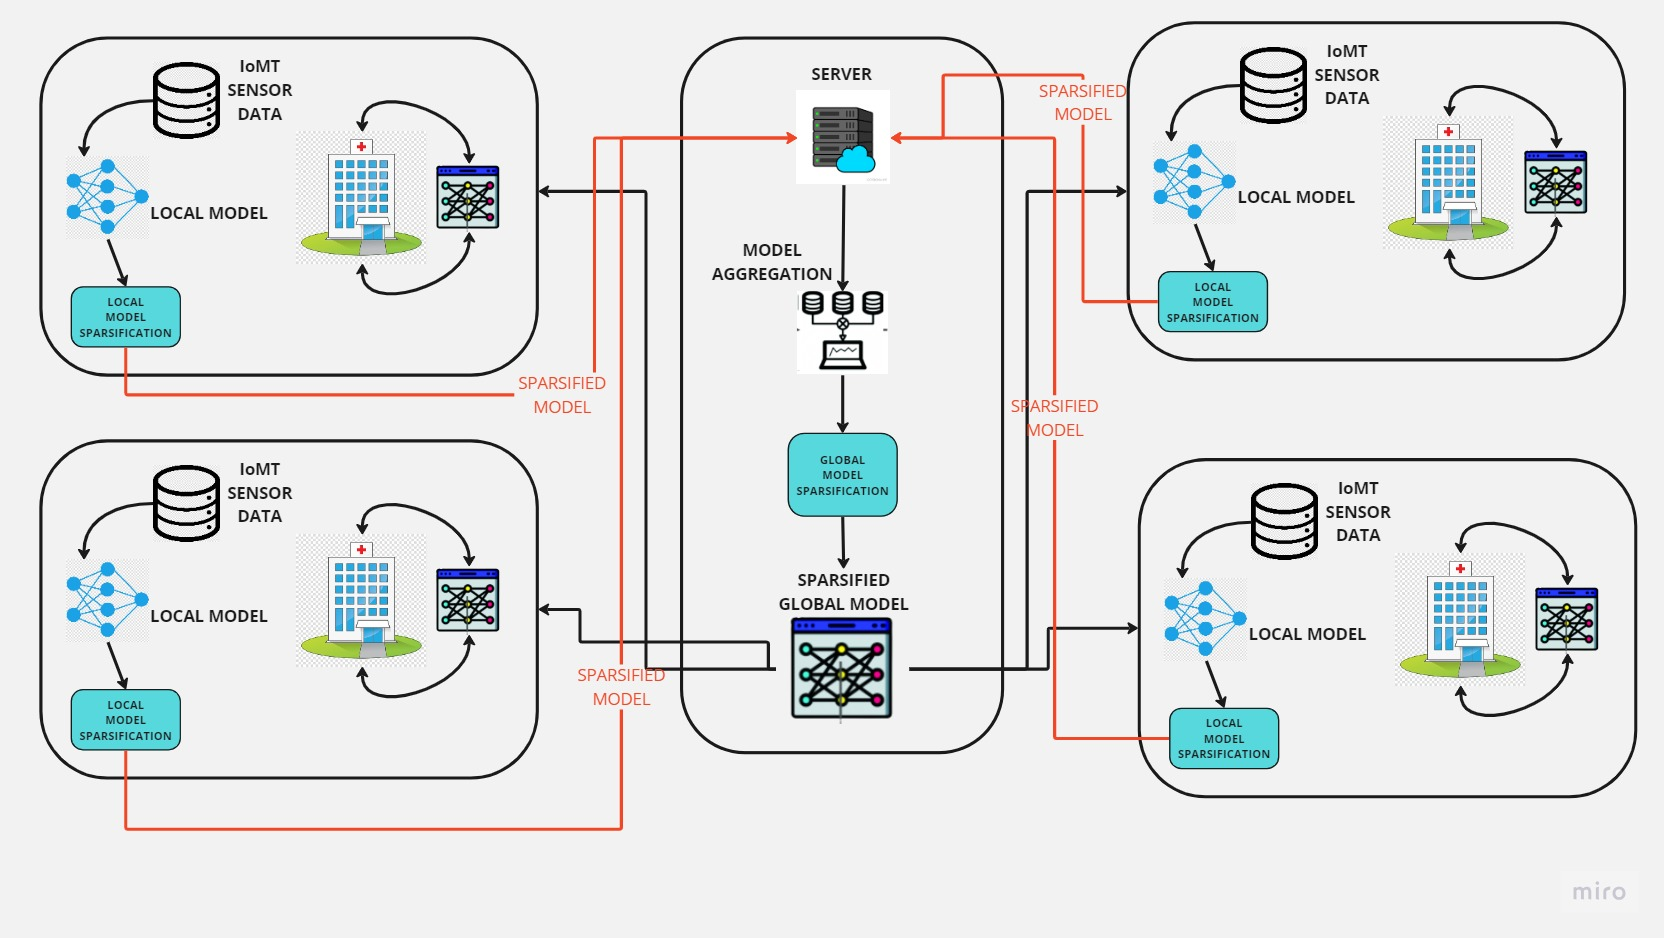
\includegraphics[scale = 0.14]{FL_ARCHITECTURE.jpg}
   % \caption{Sparsed federated learning based System Architecture}
    %\label{ds}
%\end{figure}

\section{Mathematical Model}
Federated Learning is a collaborative machine learning paradigm where a global model is refined using decentralized data sources. In this section, a mathematical model is presented that formalizes the key steps involved in the Federated Learning process. Denoting the global model as \(M\) and local models for each data holder as \(M_i\), the model encompasses initialization, local training, model parameter collection, global model updates through federated averaging, iterative refinement, and testing. This mathematical representation provides a concise framework for understanding the dynamics of Federated Learning, capturing both the training and testing phases systematically.

Let \(M\) represent the global model, and \(M_i\) the local models for each data holder indexed by \(i\).

\subsection{Initialization:}
The global model \(M\) is constructed based on globally accessible proxy data. Each data holder initializes their local model by requesting the current global model \(M\) from the server.
\[ M = \text{Initial Global Model} \]

\subsection{Local Training:}
Each data holder \(i\) trains their local model \(M_i\) using their own local data.
\[ M_i = \text{Train}(M, \text{Local Data}_i) \]

\subsection{Model Parameter Collection:}
The server collects the local model parameters periodically from all data holders.
\[ \text{Model Parameters}_i = \text{Collect}(M_i) \]

\subsection{Global Model Update:}
The server updates the global model \(M\) by federated averaging of the collected model parameters.
\begin{align*}
M &= \text{FederatedAverage}(\text{Model Parameters}_1, \\
&\quad \text{Model Parameters}_2, \\
&\quad \ldots, \\
&\quad \text{Model Parameters}_n)
\end{align*}
The federated averaging can be represented as:
\[ M = \frac{1}{n} \sum_{i=1}^{n} \text{Model Parameters}_i \]

\subsection{Iteration:}
Steps 2-4 are repeated iteratively until the global model reaches saturation.
\begin{align*}
\text{Repeat } \{ &M_i = \text{Train}(M, \text{Local Data}_i), \\
&\quad M = \text{FederatedAverage}(\text{Model Parameters}_1, \\
&\quad \quad \text{Model Parameters}_2, \\
&\quad \quad \ldots, \\
&\quad \quad \text{Model Parameters}_n) \}
\end{align*}

\subsection{Testing:}
Testing is conducted locally on the test set of each client and globally on a generic dataset.
\[ \text{Local Test Accuracy}_i = \text{Test}(M_i, \text{Local Test Set}_i) \]
\[ \text{Global Test Accuracy} = \text{Test}(M, \text{Generic Test Set}) \]
Note: Variations in local and global test accuracies may be attributed to differences in data properties among clients.



\begin{algorithm}[H]
\begin{scriptsize}  
    \SetAlgoNlRelativeSize{0}
    \SetAlgoNlRelativeSize{-1}
    \SetAlgoNlRelativeSize{1}
    \SetAlgoNlRelativeSize{-2}
    
    \textbf{Initialization:}
    \begin{itemize}
        \item Global Model Initialization: $M = \text{Initial Global Model}$
        \item Local Model Initialization: For each data holder $i$, request and initialize local model $M_i$ by training on the current global model 
        
        $M$: $M_i = \text{Train}(M, \text{Local Data}_i)$
    \end{itemize}
    
    \textbf{Iteration:}
    \While{the global model has not reached saturation}{
        \textbf{Local Training:} For each data holder $i$, update their local model: $M_i = \text{Train}(M, \text{Local Data}_i)$\;
        
        \textbf{Model Parameter Collection:} The server collects local model parameters from all data holders: $Model Parameters_i = \text{Collect}(M_i)$\;
        
        \textbf{Global Model Update:} Update the global model using federated averaging: 
        \[
            M = \frac{1}{n} \sum_{i=1}^{n} Model Parameters_i
        \]
    }
    
    \textbf{Testing:}
    \begin{itemize}
        \item \textbf{Local Testing:} For each data holder $i$, conduct testing on their local test set:

        $Local Test Accuracy_i = \text{Test}(M_i, \text{Local Test Set}_i)$
        \item \textbf{Global Testing:} Conduct testing on a generic dataset to obtain global test accuracy: 
        
        $Global Test Accuracy = \text{Test}(M, \text{Generic Test Set})$
    \end{itemize}
    
    \caption{Federated Learning Algorithm}
\end{scriptsize}
    
\end{algorithm}

Algorithm 1 illustrates an integrated learning algorithm, which is a collaborative machine learning algorithm that uses decentralized data sources. The algorithm starts with an initial phase, where a global model (M) is built based on accessible proxy data, and each database initializes its local model (Mi) by requesting the current global model from the server Through federated averaging over the global model to update the aggregated parameters. This iteration continues until the global model reaches saturation, where a local-global test is performed to verify accuracy. The algorithm emphasizes the structural dynamics of federated learning, takes both training and testing steps, and provides a concise framework for understanding its collaborative model refinement approach.

\section{Experiments and Results}

\subsection{Simulation Scenario}
The Python software platform called Kaggle is used to simulate the suggested federated learning model. The features of federated averaging, local training, and client creation are implemented in a federated SVM class. The required number of customers can be changed and adjusted according to the user. The data is automatically split into segments for the experiment based on randomness and then sent to clients for testing, validation, and training.

\subsection{Dataset}

The dataset used contains images related to COVID-19 and Viral Pneumonia. The images are loaded and processed for further analysis, including resizing to 100x100 pixels. The datasets (covid and pnemo) are created for COVID and Viral Pneumonia images, respectively. Additionally, the code checks for a specific flattened image shape (89401) for Viral Pneumonia images, which might be specific to the dataset characteristics.The code essentially loads, displays, and processes radiography images from the COVID and Viral Pneumonia categories. It involves resizing images to a standardized size (100x100 pixels) and flattening them for further analysis or model training. The specific conditions, such as the check for a flattened shape of 89401 for Viral Pneumonia images, are dataset-specific and may depend on the characteristics of the provided dataset. The processed data is then stored in NumPy arrays (covid and pnemo).

The data is automatically split among the different clients based on randomness.
\subsection{Results}
A simulation of the proposed algorithm was carried out with 3 clients and 3616 COVID data images with 1205 Viral Pneumonia images into consideration and performed 5 rounds on the dataset which was randomly divided between the clients. The parameter size was 80112 weighted matrix with 32 bias matrix for FL SVM. The same dataset was used on the normal SVM model simultaneously for comparison with the Federated SVM model. 
\begin{figure}[H]
    \centering
    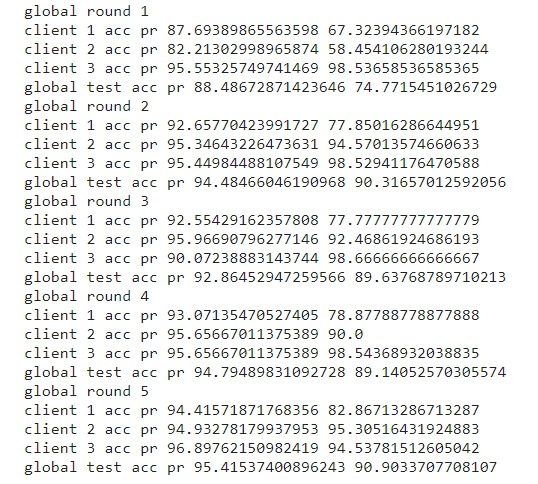
\includegraphics[scale = 0.35]{WhatsApp Image 2023-11-28 at 11.08.41_b867fcfc.jpg}
    \caption{Results after each round at local and global level}
    \label{di2}
\end{figure}
The accuracy and precision metrics from each local model using the local data are shown and also the accuracy and precision metrics at the global level by using an average aggregator after taking modified parameters from local models tested on unseen data are shown in Fig.\ref{di2}

\begin{figure*}[h!]
  \subfigure[\scriptsize Accuracy after each round at global level]{
 \label{di3}
 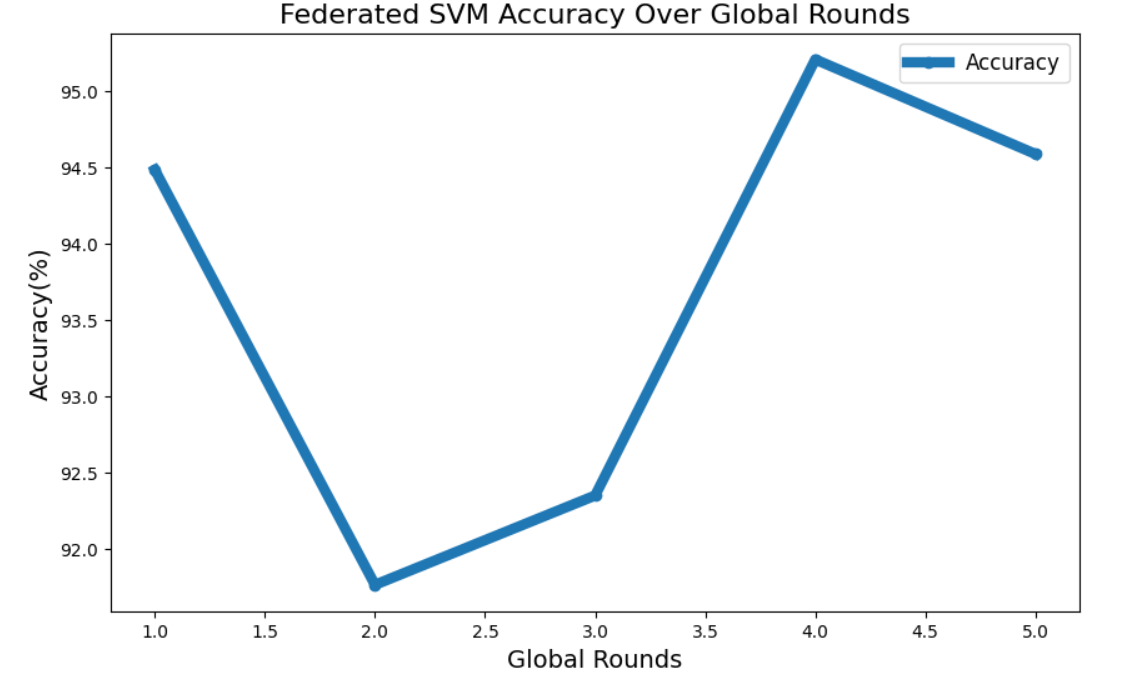
\includegraphics[scale=0.17]{plot_3.png}
 }
 \subfigure[\scriptsize Precision after each round at global level]{
 \label{di4}
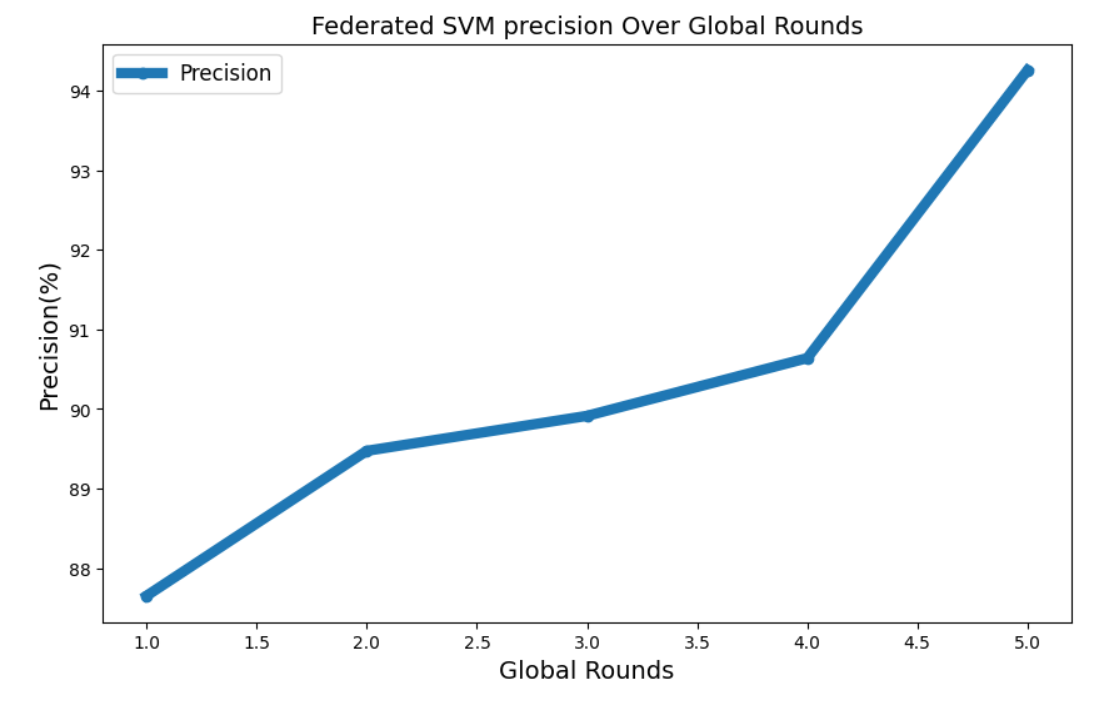
\includegraphics[scale=0.17]{plot_2.png}
}
\subfigure[\scriptsize Recall after each round at local level]{
 \label{di5}
 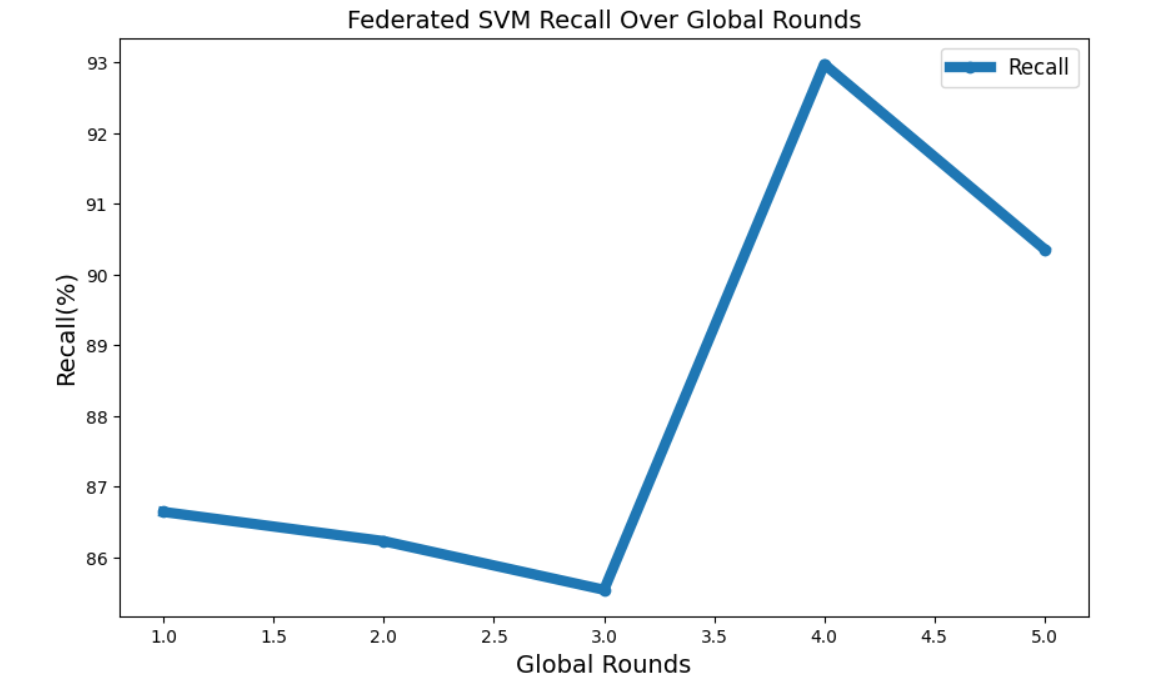
\includegraphics[scale=0.17]{plot_5.png}
 }
\subfigure[\scriptsize Individual client Accuracy after each round at local level]{
\label{di6}
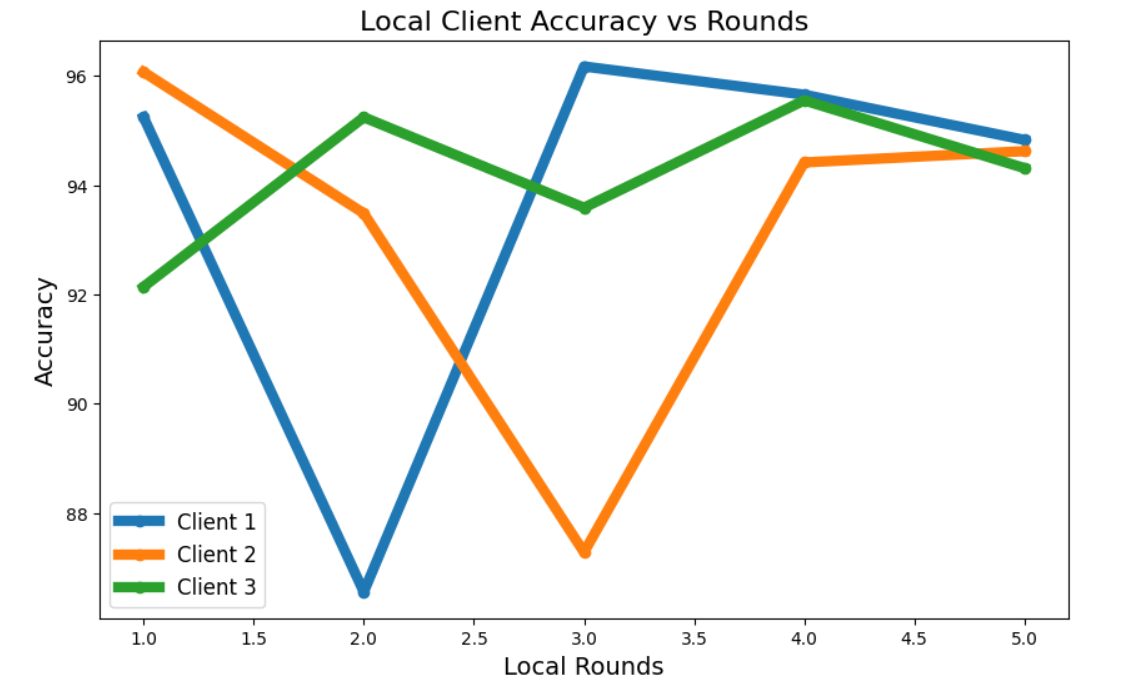
\includegraphics[scale=0.17]{plot_4.png}
}
\caption{Results: Accuracy, Precision, and Recall after each round at global and local levels}
\vspace{-0.1in}
\label{res1}
 \end{figure*}



 \begin{figure*}[h!]
 \centering
  \subfigure[\scriptsize Time taken by Federated SVM with number of rounds]{
 \label{di7}
 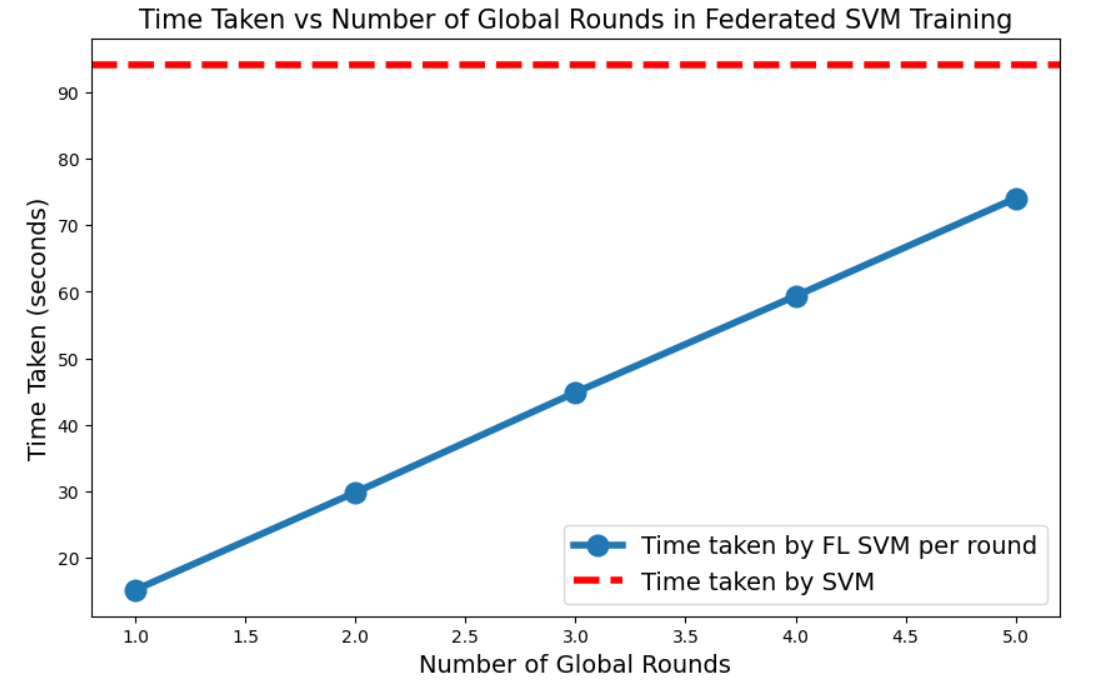
\includegraphics[scale=0.2]{plot_1.png}
 }
 \subfigure[\scriptsize Accuracy comparison between SVM and FL SVM]{
 \label{di8}
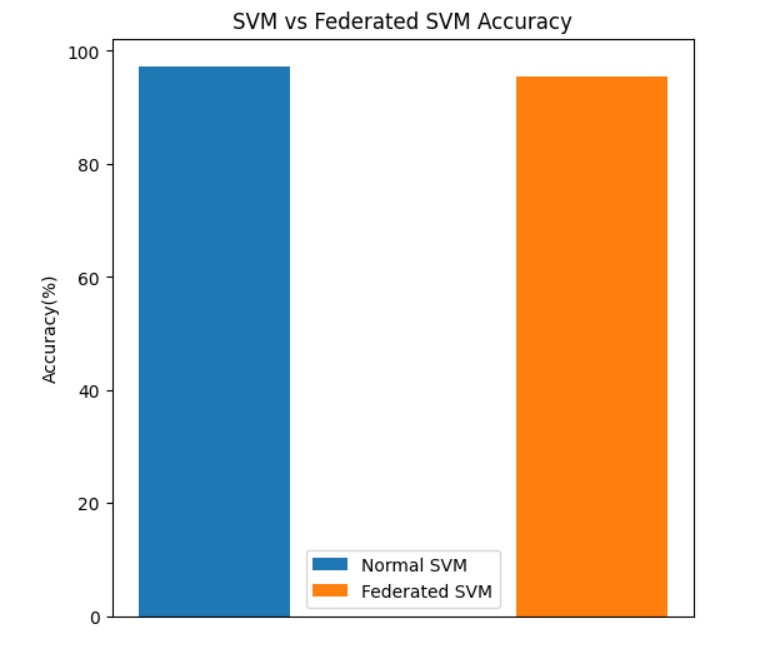
\includegraphics[scale=0.15]{WhatsApp Image 2023-11-28 at 11.59.00_22f9b447.jpg}
}
\subfigure[\scriptsize Precision comparison between SVM and FL SVM]{
 \label{di9}
 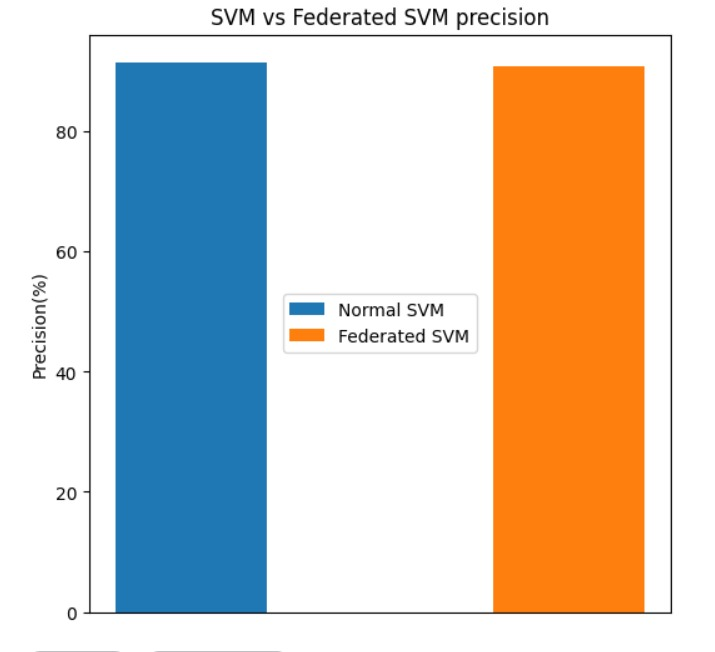
\includegraphics[scale=0.15]{WhatsApp Image 2023-11-28 at 11.59.19_afa5c1c3.jpg}
 }
\subfigure[\scriptsize Recall comparison between SVM and FL SVM]{
\label{di10}
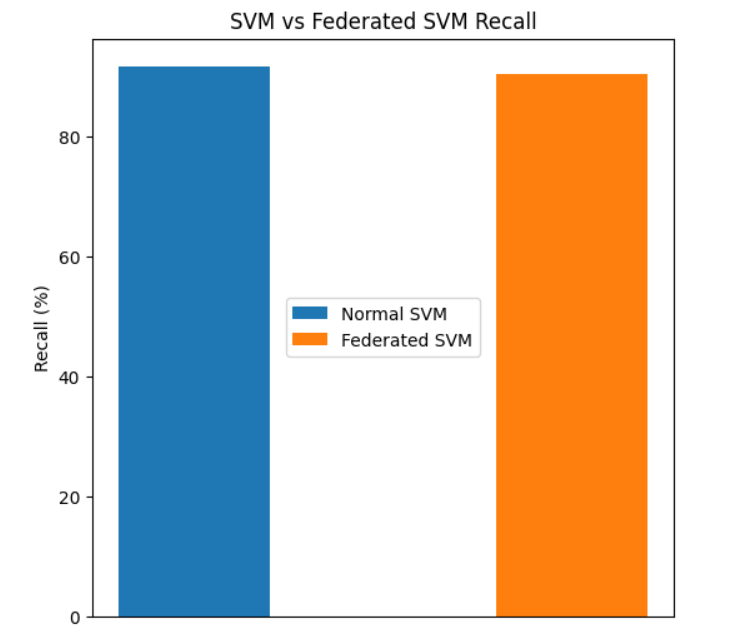
\includegraphics[scale=0.24]{plot_6.png}
}
\caption{Results: Time taken, Accuracy, Precision, and Recall comparison between SVM and FL SVM}
\vspace{-0.1in}
\label{res2}
 \end{figure*}

%\begin{figure}[htp]
 %   \centering
  %  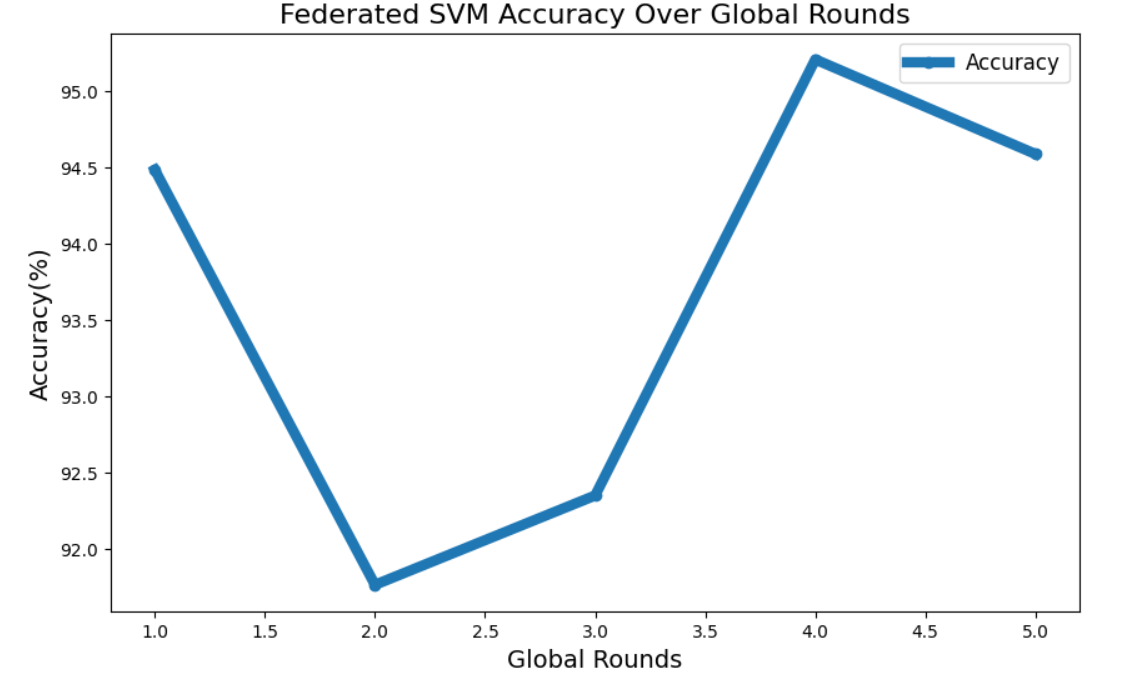
\includegraphics[scale = 0.35]{plot_3.png}
   % \caption{Accuracy after each round at global level}
    %\label{di3}
%\end{figure}
The accuracy, precision, and recall metrics after each round at the global level are plotted and shown in Fig.\ref{di3}, Fig.\ref{di4}, and Fig.\ref{di5} respectively. It can be observed that the accuracy, precision, and recall metrics values are increasing with an increase in the number of epochs or rounds.

%\begin{figure}[H]
 %   \centering
  %  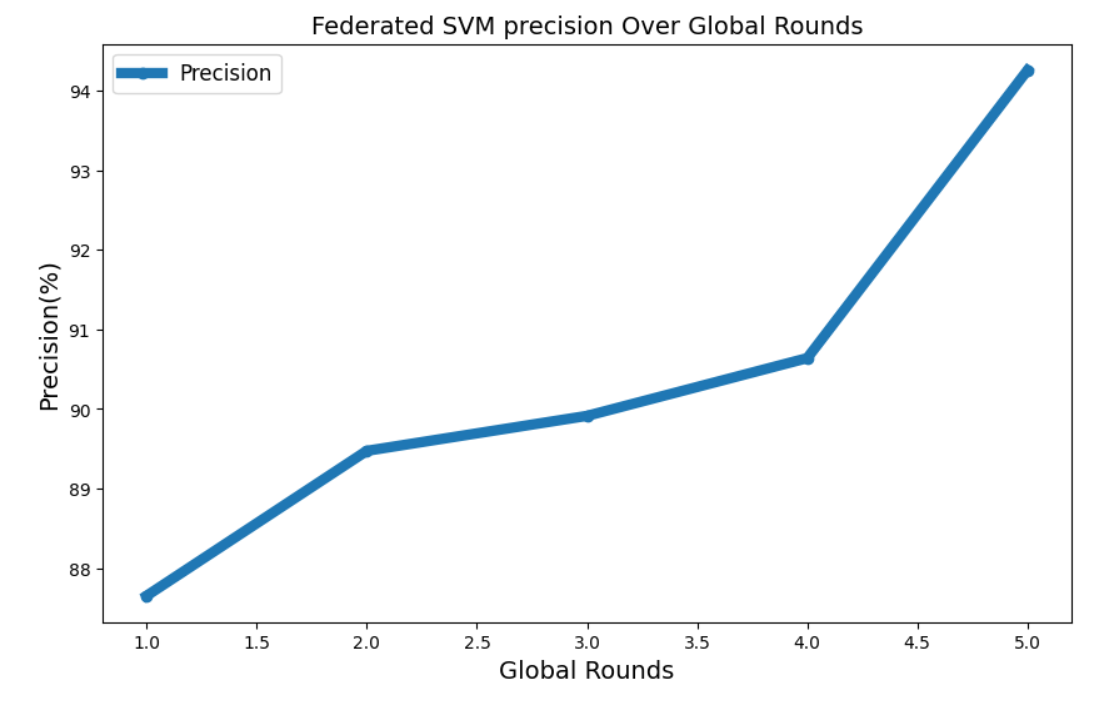
\includegraphics[scale = 0.35]{plot_2.png}
   % \caption{Precision after each round at global level}
   % \label{di4}
%\end{figure}

%\begin{figure}[H]
 %   \centering
  %  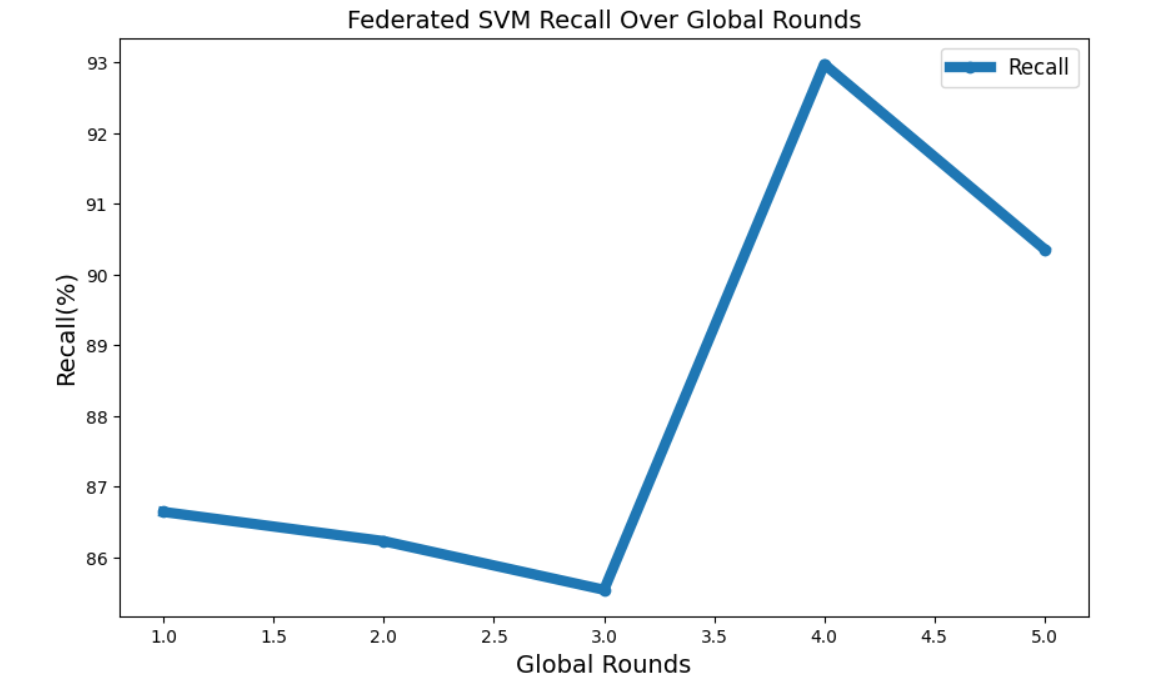
\includegraphics[scale = 0.35]{plot_5.png}
   % \caption{Recall after each round at local level}
    %\label{di5}
%\end{figure}

Fig.\ref{di6} shows how the accuracy of each participating client 
varies after each round as the data used by them will be their local data respectively. Thus there are fluctuations in accuracy which can be observed by some clients, but overall the accuracy by each client as the number of rounds increases. In Fig.\ref{di7} Federated Learning SVM time taken for each round is almost a linear function of several rounds can be seen.

%\begin{figure}[!htbp]
 %   \centering
  %  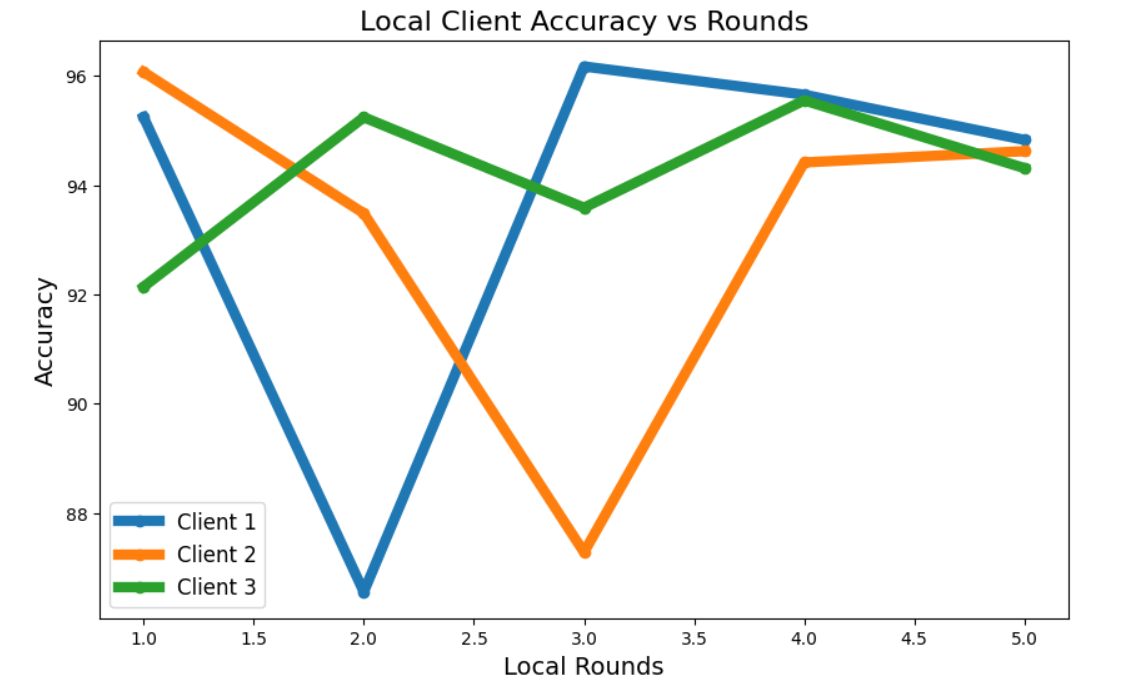
\includegraphics[scale = 0.36]{plot_4.png}
   % \caption{Individual client Accuracy after each round at local level}
    %\label{di6}
%\end{figure}

% \begin{figure}[!htbp]
%     \centering
%     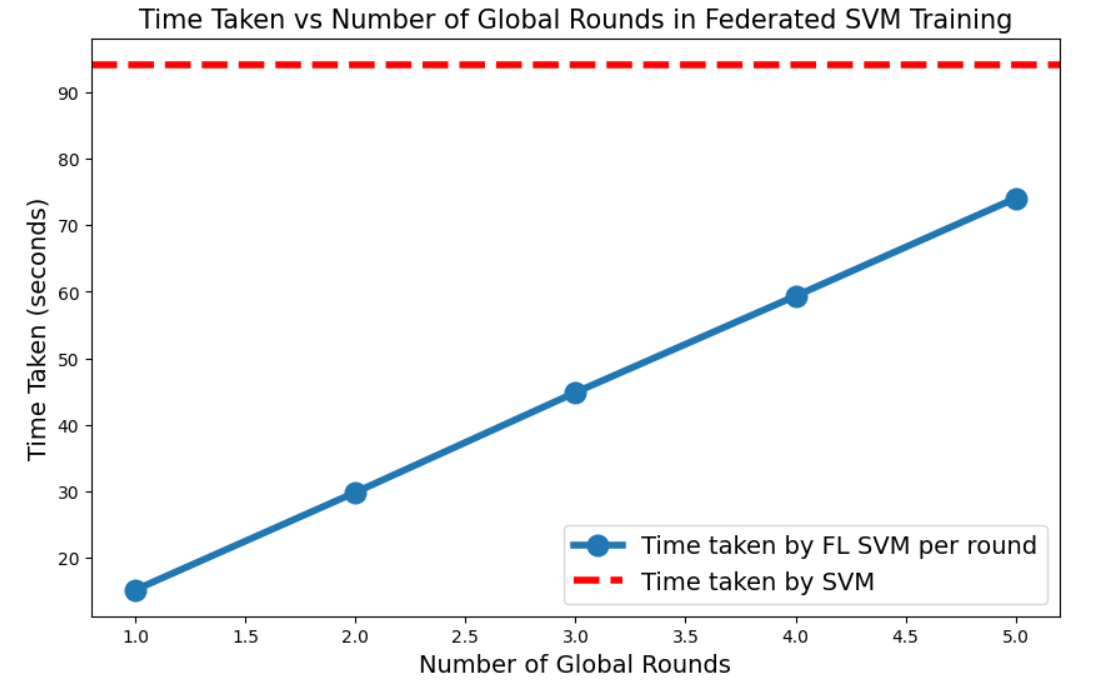
\includegraphics[scale = 0.37]{plot_1.png}
%     \caption{Time taken by Federated SVM with number of rounds}
%     \label{di7}
% \end{figure}


% \begin{figure}[H]
%     \centering
%     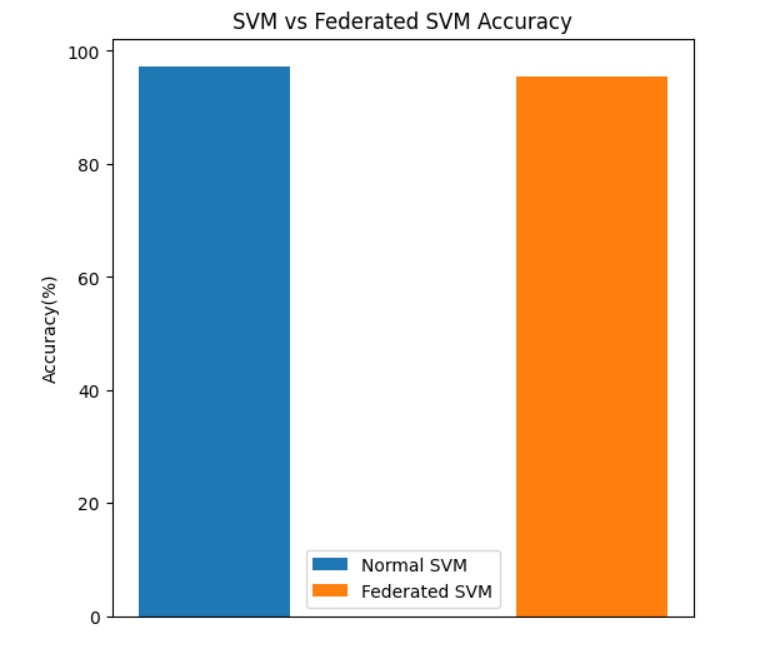
\includegraphics[scale = 0.27]{WhatsApp Image 2023-11-28 at 11.59.00_22f9b447.jpg}
%     \caption{Accuracy comparison between SVM and Federated learning SVM}
%     \label{di8}
% \end{figure}
% \begin{figure}[H]
%     \centering
%     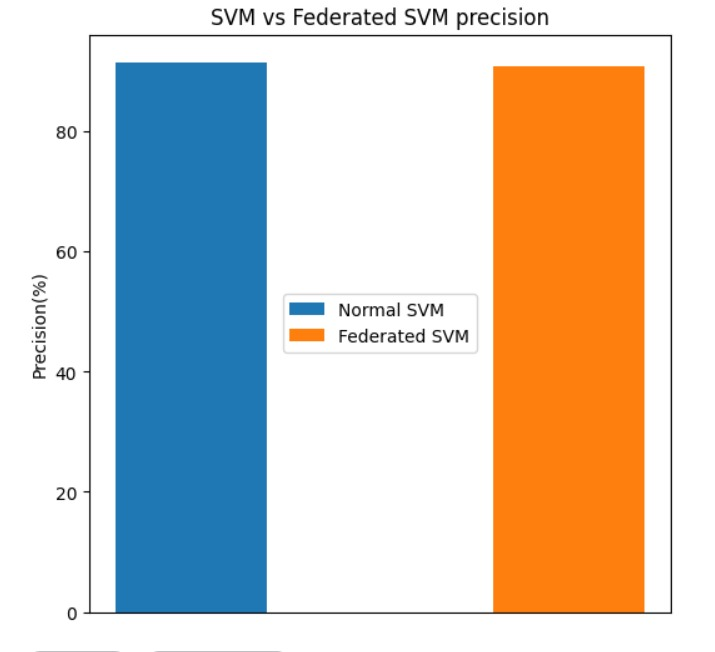
\includegraphics[scale = 0.27]{WhatsApp Image 2023-11-28 at 11.59.19_afa5c1c3.jpg}
%     \caption{Precision comparison between SVM and Federated learning SVM}
%     \label{di9}
% \end{figure}
% \begin{figure}[H]
%     \centering
%     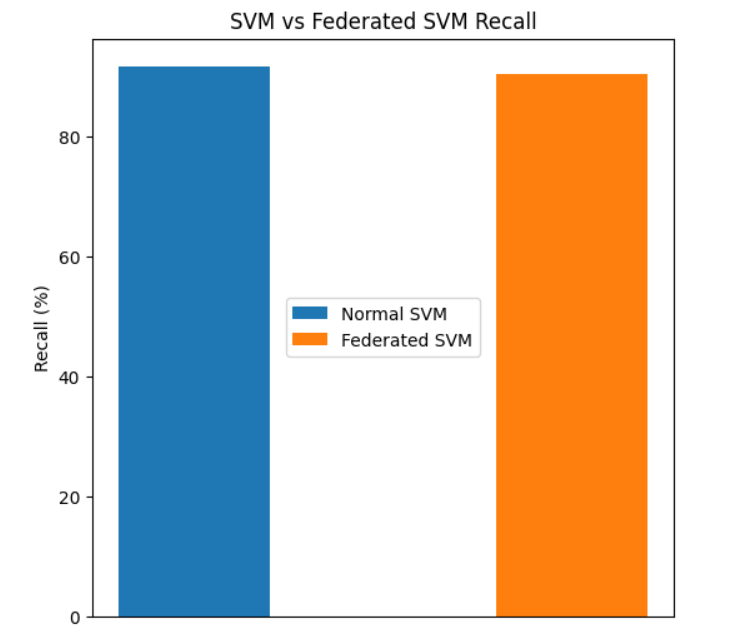
\includegraphics[scale = 0.46]{plot_6.png}
%     \caption{Recall comparison between SVM and Federated learning SVM}
%     \label{di10}
% \end{figure}

A comparative analysis is carried out between the metrics obtained by using the normal SVM model and the Federated learning SVM model. From Fig.\ref{di8}, Fig.\ref{di9}, and Fig.\ref{di10}, it can be observed that both models' accuracy, precision, and recall metrics are almost equal. Thus, the federated learning SVM model performs equally better with the SVM model while also maintaining the privacy of the data as it only shares the parameters.

\section{Conclusion and Future Works}
In this research, an exploration into federated learning, utilizing a dataset focused on Covid-Pneumonia images, is underway. The core aim of the study is to evaluate the effectiveness of the federated algorithm, with a focus on privacy and security considerations. This evaluation is carried out using a well-established dataset, and the experimentation involves three distinct clients, each equipped with its unique dataset distribution. An intriguing observation emerges when the model is tested exclusively on the local data of each client: the accuracy is notably lower. However, a pivotal improvement is witnessed with the incorporation of federated averaging into the training process. Remarkably, the accuracy achieved through federated learning is more or equal to that obtained through conventional centralized training methods. Investigating the impact of different sparsity levels on model performance and resource utilization could be a valuable avenue for future research.

%Investigating the impact of different sparsity levels on model performance and resource utilization could be a valuable avenue for future research. This not only contributes to the academic discourse on the subject but also provides practical insights for researchers and practitioners aiming to enhance the capabilities of federated learning in medical applications. Thus the investigation, mathematical design, and simulation of a sparsed federated learning model would be the future extendable works.

\section*{Acknowledgements} The work is supported by the Indian Institute of Information Technology Raichur, Karnataka, India, and is partially funded by the Brazilian National Council for Scientific and Technological Development - CNPq, via Grant No. 306607/2023-9. Ashit Kumar Dutta would like to express sincere gratitude to AlMaarefa University, Riyadh, Saudi Arabia, for providing funding to conduct this research.

\begin{thebibliography}{1}
\bibitem{1}Rani S, Kataria A, Kumar S, Tiwari P. Federated learning for secure IoMT-applications in smart healthcare systems: A comprehensive review. Knowledge-Based Systems. 2023 May 22:110658.

\bibitem{2}Gupta L. Collaborative Edge-Cloud AI for IoT Driven Secure Healthcare System. In2023 IEEE International Systems Conference (SysCon) 2023 Apr 17 (pp. 1-8). IEEE.

\bibitem{3}Ghosh S, Ghosh SK. FEEL: FEderated Learning Framework for ELderly Healthcare Using Edge-IoMT. IEEE Transactions on Computational Social Systems. 2023 Jan 23.

\bibitem{4}Prasad VK, Bhattacharya P, Maru D, Tanwar S, Verma A, Singh A, Tiwari AK, Sharma R, Alkhayyat A, Țurcanu FE, Raboaca MS. Federated learning for the internet-of-medical-things: A survey. Mathematics. 2022 Dec 28;11(1):151.
\bibitem{10} Chavhan, S., Kumar, S., Gupta, D., Alkhayyat, A., Khanna, A. and Manikandan, R., 2023. Edge-Empowered Communication-based Vehicle and Pedestrian Trajectory Perception System for Smart Cities. IEEE Internet of Things Journal.
\bibitem{5}Han B, Jhaveri R, Wang H, Qiao D, Du J. Application of robust zero-watermarking scheme based on federated learning for securing the healthcare data. IEEE journal of biomedical and health informatics. 2021 Oct 29.

\bibitem{6}Hayyolalam V, Aloqaily M, Özkasap Ö, Guizani M. Edge intelligence for empowering IoT-based healthcare systems. IEEE Wireless Communications. 2021 Jun;28(3):6-14.

\bibitem{7}Gadekallu TR, Alazab M, Hemanth J, Wang W. Guest editorial federated learning for privacy preservation of healthcare data in internet of medical things and patient monitoring. IEEE Journal of Biomedical and Health Informatics. 2023 Feb 1;27(2):648-51.
\bibitem{11} Prabhakaran, P., Chavhan, S., Kumar, M. and Rodrigues, J.J., 2023, June. ML-based Minimization of AoI in a Vehicular Communication Network. In 2023 8th International Conference on Smart and Sustainable Technologies (SpliTech) (pp. 1-6). IEEE.

\bibitem{8}Truex S, Baracaldo N, Anwar A, Steinke T, Ludwig H, Zhang R, Zhou Y. A hybrid approach to privacy-preserving federated learning. InProceedings of the 12th ACM workshop on artificial intelligence and security 2019 Nov 11 (pp. 1-11).

\bibitem{9}Wen D, Li X, Zhou Y, Shi Y, Wu S, Jiang C. Integrated Sensing-Communication-Computation for Edge Artificial Intelligence. arXiv preprint arXiv:2306.01162. 2023 Jun 1.

\bibitem{12} Chavhan, S., Gupta, D., Alkhayyat, A., Alharbi, M. and Rodrigues, J.J., 2023. AI-Empowered Game Theoretic-Enabled Dynamic Electric Vehicles Charging Price Scheme in Smart City. IEEE Systems Journal.

\end{thebibliography}
\end{document}
